% begin module even-power-functions
\begin{frame}
\begin{tabular}{cc}
\ \only<handout:0| -2>{%
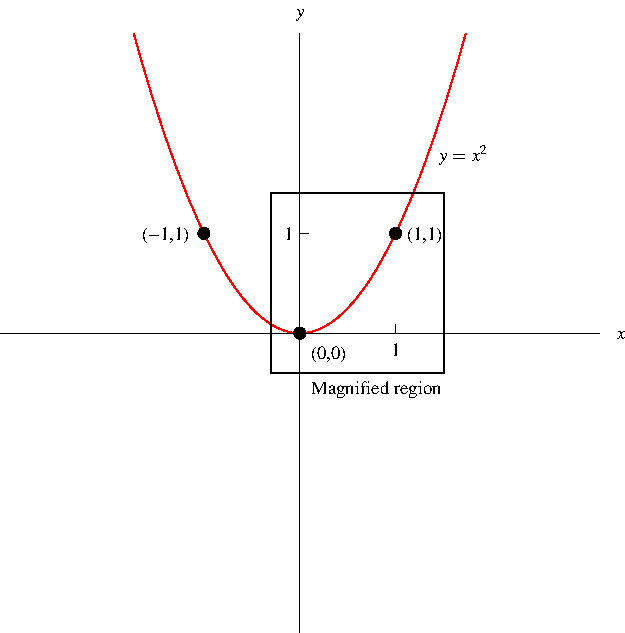
\includegraphics[height=5cm]{precalculus/pictures/01-02-evenpowersa.pdf}%
}%
\only<handout:0| 3>{%
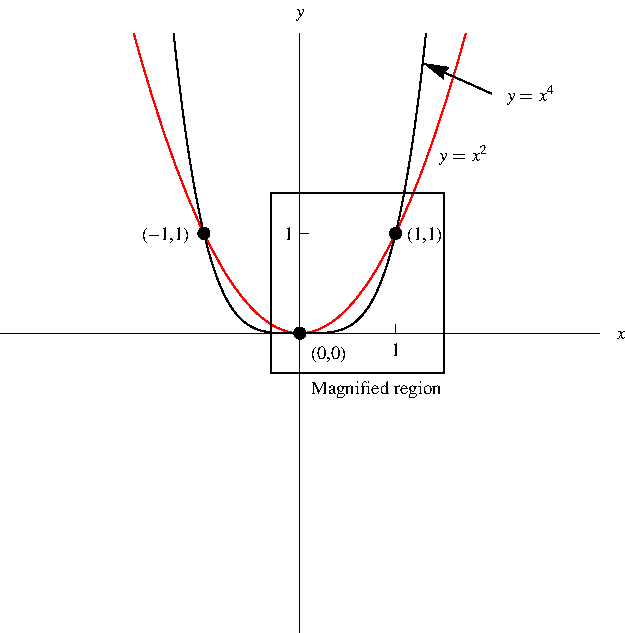
\includegraphics[height=5cm]{precalculus/pictures/01-02-evenpowersb.pdf}%
}%
\only<4>{%
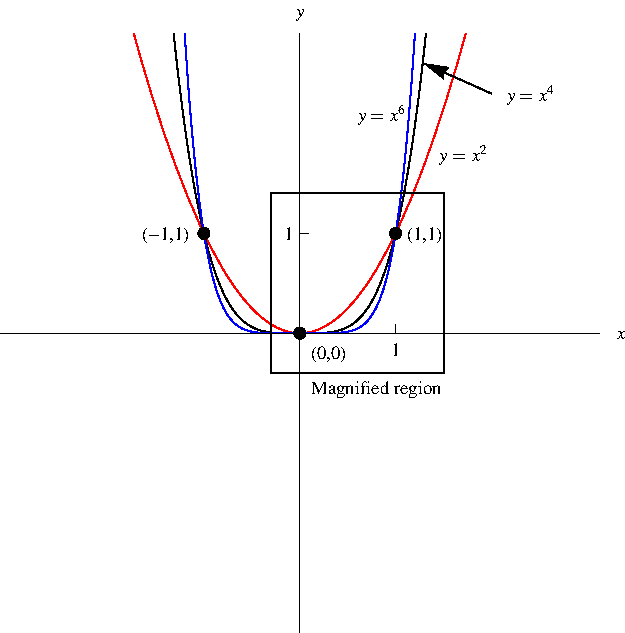
\includegraphics[height=5cm]{precalculus/pictures/01-02-evenpowersc.pdf}%
}%
&%
\ \only<handout:0| -2>{%
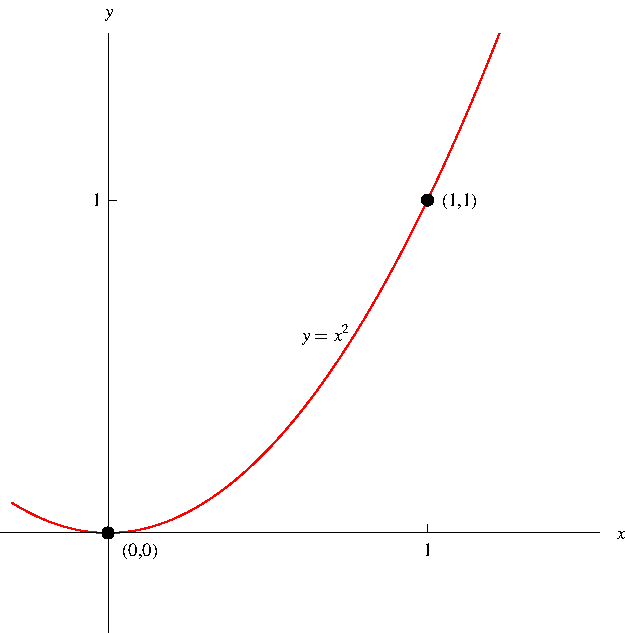
\includegraphics[height=5cm]{precalculus/pictures/01-02-evenpowerszooma.pdf}%
}%
\only<handout:0| 3>{%
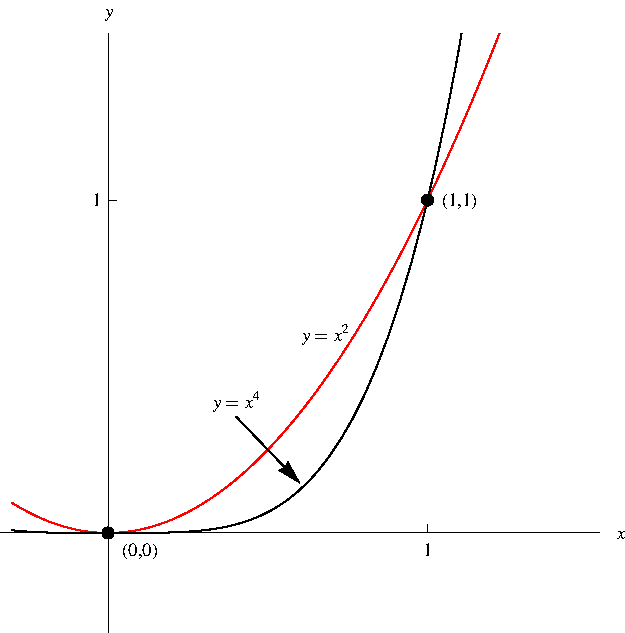
\includegraphics[height=5cm]{precalculus/pictures/01-02-evenpowerszoomb.pdf}%
}%
\only<4>{%
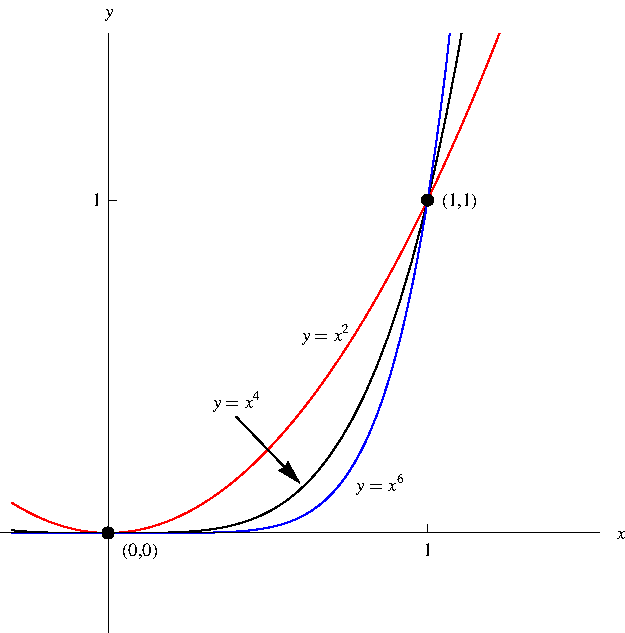
\includegraphics[height=5cm]{precalculus/pictures/01-02-evenpowerszoomc.pdf}%
}%
\end{tabular}
\begin{itemize}
\item<2->  All positive, even powers of $x$ (e.g., $x^2, x^4, \ldots$) pass through $(0,0), (-1, 1)$, and $(1,1)$.
\item<3->  If $n > m$, then $y = x^n$ is higher than $y = x^m$ when $x > 1$ or when $x < -1$, but lower when $-1 < x < 1$.
\end{itemize}
\end{frame}
% end module even-power-functions
